\section{Project Management}\label{sec:projectmanagement}
To implement the system we choosed web platform since it will be easier to use with any kind of devices. It will requires only a browser and internet to use the application and one can use it from anywhere at anytime he wishes to. The application will require a frontend which is to interact with it's user through browser and backend which will perform functionalities and some will make some operations into the database based on the query that is selected by the user.\\
Developing this application would requires a huge time if we would have wished to complete it individually. So we initially planned to split the entire project into certain branches with small or medium scaled tasks and distribute them among all of our teammates. After the completion we planned to assemble all the branches from our teammates and merge them together to build the final system successfully. It is clearly visible that we were moving forward with Scrum\footnotemark method while completing the project. Following scrum model provision we made following 5 steps or phases mentioned below to execute our project. 
\begin{enumerate}
\item \textbf{Product Backlog Creation}\\
In this process, we transformed the significance and functional details of the system into short stories\\ 
If we think of a regular student being whose semester final exam is in a few days, has to pay the semester fee in a specific time period set by the administrator. This causes students suffering and directly effects on their preparation. Besides, in conventional way of transaction, university is fully dependent on one specific bank branch which causes an exhausting and tormenting situation when a huge number of students wishes to pay the fees on the same day. Many students even fail to submit the fee on time as they can't make any transaction on non-working hours. Teachers are also recorded to lose about one-third of the course period in taking attendance manually which effects on the concentration of students. On the other hand administration often find it tiresome to update data of students manually in papers. It not only consumes huge time, but also requires physical presence of a good number of person to complete. \\
These reasons influenced our team to develop a single application with the knowledge of our database course that is able to solve all of the issues mentioned above.


\item \textbf{Sprint planning and creating backlog}\\

The next stage was to do the sprint backlog creation for which our team had to select the important user stories and made them into smaller tasks. We made plans on how to get the task completed. Also, our team did prioritize the necessary tasks to accomplish the project more smoothly. The sprint duration lasted about 9 to 10 days which was long enough to allow the developer to work thoroughly. 

\item \textbf{Working on sprint}\\

This was a practical phase. The actual stories were moved as small tasks in the sprint backlog where the actual work started. To begin with, a task board also called Kanban board in Trello\footnotemark was made with a lot of cards in used. The cards used to specify the details about the tasks such as assignee, work details, due date or the time duration, etc. This cards also were used to record our meeting schedule and details as well as future updates. The task board consisted of the following columns the "To Do" lists, "Work In Progress" and then "Testing" and "Work Done" columns. A typical task board is shown in the diagram below.
\\

In scrum method, a project is usually done through merging the contributions of a whole team being led a leader among them. In our case, Md Masud Majumdar was the leader among us, who planned and led the team from beginning to end. Each team member had contributed in parts of the entire project.\\

We held regular virtual meetings where all the teammates together, came up with all the various ideas to design the database schema. The meetings we held virtually through Google Meet\footnotemark and Zoom software were led by Tareq Rahman Khan. Within a week, we decided to draw the first E-R Diagram on our ideas which was fianlly done by Palash Hossen. Later it was modified by Nu Sai Mong Marma.\\

While developing the system, we used Github\footnotemark to make the collaboration among teammates and to integrate all the assigned task and make the final system. Github not only allowed us to collaborate with our teammates but also to control the modifications of the application. Since the start of the project, our team made about 100 of commits into Github repository. All the commits are from Tonmoy Chandro Das and Md. Masud Majumdar as frontend and backend funcionalities were developed by them. To interact with github, we used git in our local machine and Visual Studio Code as code editor.\\

While developing the system, we also looked after about the documentation of this entire project. This documentation was prepared under the leadership of Hamza Mohtadee.\\

\begin{figure}[H]
    \centering
    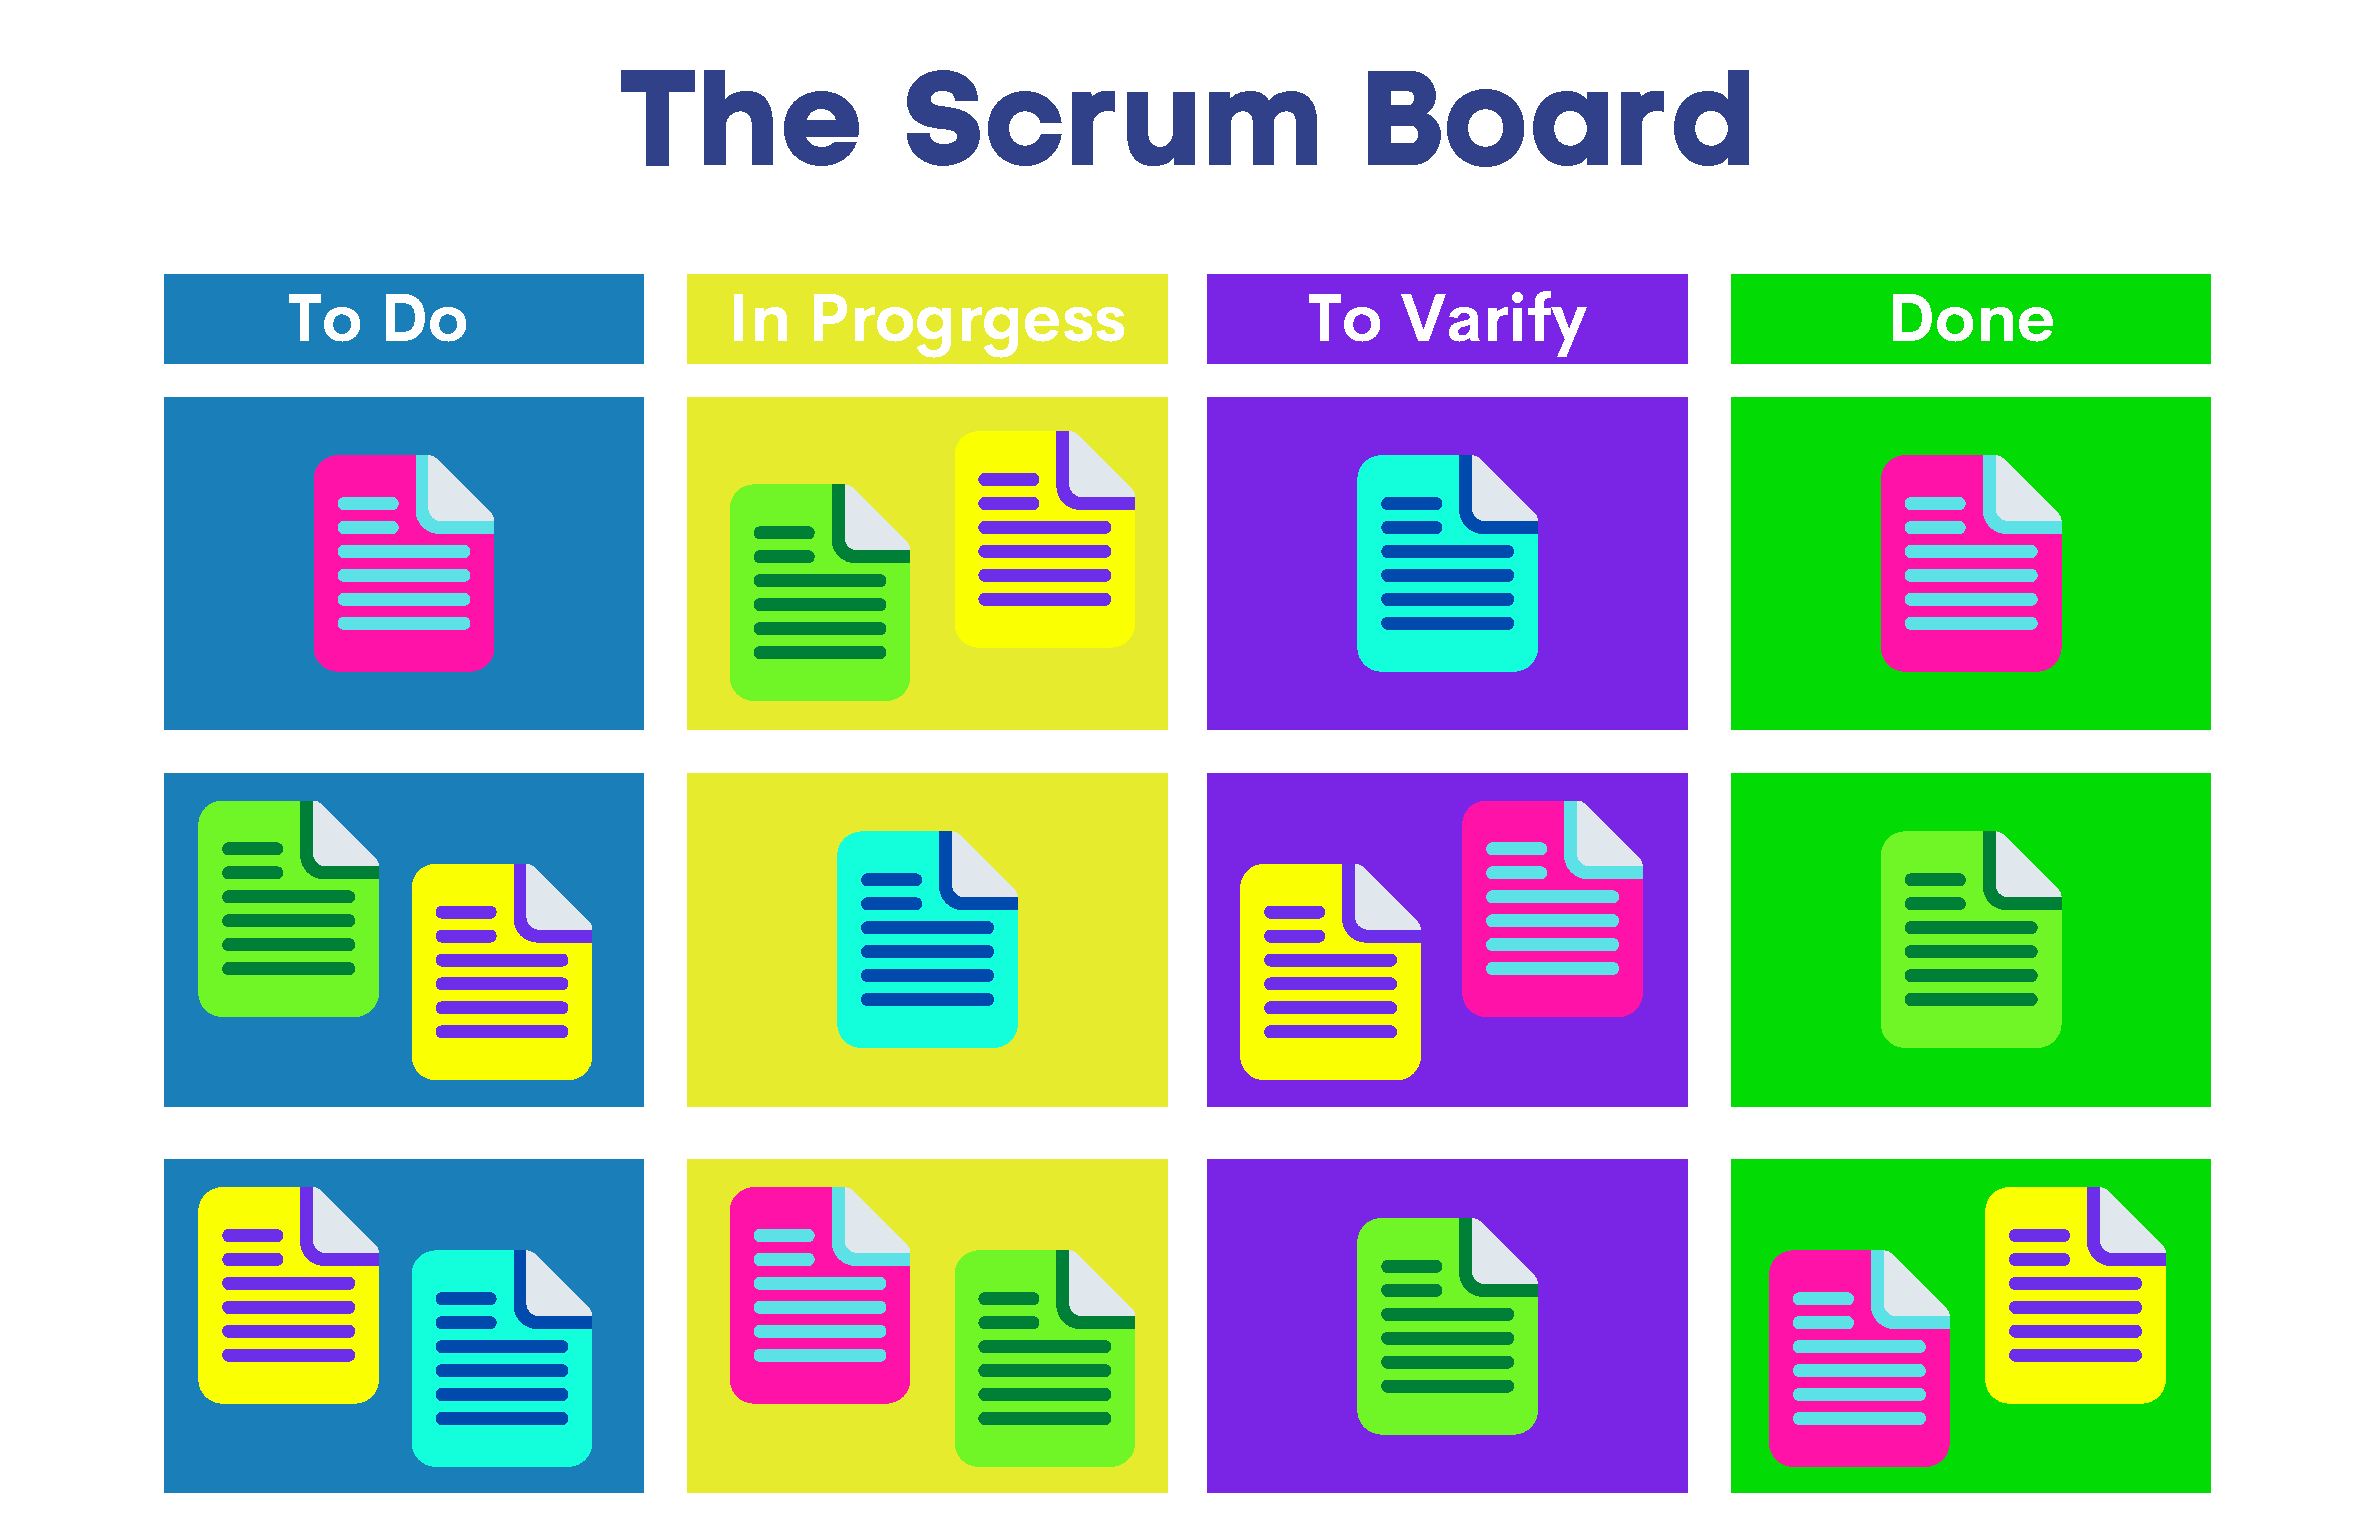
\includegraphics[width=1\textwidth]{images/scrum_board}
    \caption{Project Management Agile Scrum Board Template}
    \label{fig:scrum_board}
\end{figure}

\item \textbf{Testing and Product Demonstration}\\

This phase is basically the modification phase based on the review of stack holders of our system. The tasks completed were to be realized as a working product with full life cycle testing. Every sprint that was completed was demonstrated to the stack holders i.e. students, teachers and concerned authority for their acceptance and their viewpoint on the complete solution. We received cordial reviews from the stack holders and in most of the cases they expressed their pleasures on the solution given by us. Being asked for suggestion, a part of them gave us some suggestion for modifications on several parts of the application. We obviously implemented many of those and integrated to the final system.

\item \textbf{Retrospective and the next sprint planning}\\

The result of this step was to discuss what had gone well and what could be improved for the next level. Also we discussed the lessons learned and the pitfalls of any particular issues or problems related to this project. We planned our next sprint that is future work. We aim to integrate more functions into the system and withing a time, make it a reliable fully functioned university management system. With the current knowledge and more study, our team is quite confident to make that possible. This will results a paperless administration. All the official tasks will require less time than ever. In the meantime, we will assuredly maintain the system to make it an uninterrupted service provider application.


\end{enumerate}

From the beginning of the planning to the final execution of the system, each and every member of our team has equally likely contributed to the project. We tried to make a better system than current one and it was finally possible as together all of us went through hundreds of ideas. We tried to make the best use of current technologies to complete this project. During the progress, we learned a lot of new things while being stuck on problems we faced never before. Without proper project management principles, projects could be handled haphazardly and are at a much higher risk of project failure, delay in the project, and being over budget. Knowing the fundamentals of project management improved our chances of completing a project successfully. 

\footnotetext[1]{Scrum is an agile development methodology used in the development of Software based on an iterative and incremental processes. Scrum is adaptable, fast, flexible and effective agile framework that is designed to deliver value to the customer throughout the development of the project.}

\footnotetext[2]{Trello is a web-based, Kanban-style, list-making application and is developed by Trello Enterprise, a subsidiary of Atlassian. It is a visual collaboration tool that enables one to organize and prioritize projects in a fun, flexible, and rewarding way. A Trello board is a series of lists, with a bunch of cards attached and packed full with powerful features and automation. [website: www.trello.com]}

\footnotetext[3]{Google Meet is a video-communication service developed by Google. It is one of two apps that constitute the replacement for Google Hangouts, the other being Google Chat. website[www.meet.google.com]}

\footnotetext[4]{GitHub is a provider of Internet hosting for software development and version control using Git. It offers the distributed version control and source code management functionality of Git, plus its own features. It lets us and others work together on projects from anywhere. [website: www.github.com]}

\clearpage